\documentclass[12pt]{article}
\usepackage[utf8]{inputenc}
\usepackage{polski}
\usepackage{hyperref}
\usepackage{listings}
\usepackage{mathtools}
\usepackage{graphicx}
\usepackage{fullpage}
\usepackage{enumerate}
\usepackage{float}
\usepackage{caption}
\usepackage{parskip}
\usepackage{subcaption}
\title{Teoria i Inżynieria Ruchu Teleinformatycznego \\ Sprawozdanie z projektu}
\author{Ewelina Kawecka (201420) \\ Michał Smyk (203254)}
\graphicspath{ {gfx/} }
\begin{document}
\maketitle
\thispagestyle{empty}
\clearpage
\setcounter{page}{1}

\section{Wstęp}
Celem całości projektu było stworzenie programu, który na podstawie historii ruchu w sieci komputerowej będzie w stanie przeanalizować go pod kątem interesujących właściwości, które mogą być w tej historii zawarte. Projekt podzielony został na dwie części. Pierwsza część projektu jest odpowiedzialna za ekstrakcję danych z plików PCAP, zawierających nagrane informacje na temat historii ruchu w sieci. Druga część projektu ma za zadanie na podstawie otrzymanych danych wyekstraktować kod html a następnie przetworzyć go pod kątem częstotliwości występowania elementów takich jak: rozszerzenia obrazków, klasy html, tagi html, rodzaje linków. Dodatkowym zadaniem proponowanej aplikacji jest wydobywanie z otrzymywanych danych obrazków i zapis ich w pamięci. 

\section{Opis problemu}
Głównym problemem, na którym skupia się pierwsza część projektu jest ekstrakcja i filtrowanie danych zawartych w pliku PCAP. Z racji, że w plikach tych znajdują się również dodatkowe informacje, które ze względu na brak przydatności do celów zadania powinny zostać odfiltrowane. Pozostałe dane, które przechowują przydatne informacje powinny zostać przetworzone w taki sposób, aby umożliwić odczytanie z nich informacji, które interesują osobę wykorzystującą program. Filtracja i ekstrakcja danych podzielona została na kilka etapów, które w postaci funkcji udostępniane są przez program. Funkcje te przedstawia rysunek \ref{img:funkcje}.

\begin{figure}[h]
\centering
\caption{Atomowe funkcje opracowane w ramach pierwszej części projektu}
\label{img:funkcje}
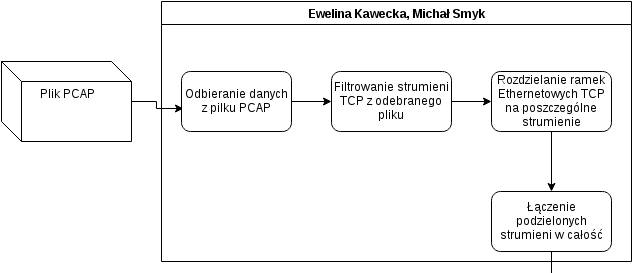
\includegraphics[width=0.7\textwidth]{Wykres.png}
\end{figure}


Odfiltrowane i przetworzone dane muszą zostać następnie poddane kolejnemu procesowi, którego zadaniem jest wydobycie kodu html w czystej postaci. Podczas ekstrakcji html należy również zwrócić uwagę na kompresję danych i w przypadku jej wystąpienia konieczne jest odpowiednia dekompresja kodu. 
Tak przygotowane dane poddawane są później m.in. analizie statystycznej. 

Zgodnie z zaleceniami prowadzącego każda atomowa funkcja realizowana przez program udostępniona jest w formie usługi - szczegółowe informacje na ich temat dostępne są w rozdziale \ref{dzialanie}. 

\section{Opis implementacji programu}
\label{dzialanie}
...
\subsection{Ekstrakcja HTML}
Tak spreparowane dane przesyłane są następnie do pliku html\_extractor.py, w którym odbywa się wydobywanie kodu html. 
Ponieważ aplikacja ma za zadanie analizować ruch internetowy należy brać pod uwagę tylko dane przesyłana na porcie 80. Ze względu na fakt, że interesują nas tylko odpowiedzi serwera omawiany moduł ignoruje treść samych zapytań. Odczytanie danych jest możliwe dzięki wykorzystaniu biblioteki dpkt. Dekompresja danych odbywa się przy pomocy biblioteki gzpi po uprzednim sprawdzeniu zawartości nagłówka 'content-encoding'. Zadaniem modułu jest również ekstrakcja obrazków. Osiągane jest to poprzez weryfikacje nagłówka 'content-type', jesli nagłówek ten zawiera wartości typowe dla obrazów to aplikacja zapisuje otrzymany obraz w dedykowanym folderze. Ostatecznie moduł przesyła dane dalej do pliku html\_receiver.py, którego zadaniem jest właściwie tylko dalsze przekazanie kodu do usług odpowiedzialnych za analizę statystyczną.

\subsection{Analiza HTML}
Analiza każdej z zaimplementowanych właściwości kodu HTML jest realizowana przez dwa oddzielne pliki: plik serwera - zajmujący się odbieraniem danych oraz plik analizujący - odpowiedzialny za samo przetwarzanie danych. 

\section{Opis usług}

\subsubsection{DataExtraction/html\_extractor.py} 
%\mbox{}\\
\textbf{Komunikuje się z usługami:}\\
\begin{itemize}
\item DataAnalysys/html\_receiver.py
\end{itemize} 

\section{Przykładowe wywołanie}
Program wywołujemy poprzez uruchomienie wszystkich usług, które składają się na jego elementy:
%\begin{itemize}
%\item main.py
%\item frame filter.py
%\item merger.py
%\item receiver.py
%\end{itemize}

%Dopiero po uruchomieniu tych plików, możemy za pomocą pliku \emph{sender.py} wysłać plik z rozszerzeniem %\emph{.pcap} jako pierwszy argument, aby wysłać zadany plik do poszczególnych usług w celu ich dalszego %przetworzenia. 
\end{document}
